\documentclass[../../../doc/main]{subfiles}
\begin{document}
    \setcounter{chapter}{6}
    \setcounter{section}{2}
    \section{解説}\label{解説6}
    \begin{itemize}
        \item [(1)]
            右に図を示す。立方体の表面のうち上面を除く面が$S$である。
            \begin{mawarikomi}{}{
                \tdplotsetmaincoords{70}{60}
                \begin{tikzpicture}[tdplot_main_coords,scale=1.5]
                    %\shadedraw[tdplot_screen_coords,ball color = white] (0,0) circle (1.732);
                    \coordinate (O) at (0,0,0);
                    \coordinate (A) at (1,1,-1);
                    \coordinate (B) at (-1,1,-1);
                    \coordinate (C) at (-1,-1,-1);
                    \coordinate (D) at (1,-1,-1);
                    \coordinate (E) at (1,1,1);
                    \coordinate (F) at (-1,1,1);
                    \coordinate (G) at (-1,-1,1);
                    \coordinate (H) at (1,-1,1);
                    %\draw [white] (0,0,0) -- (0,0,-3);
                    \fill [opacity=.1] (A) -- (B) -- (C) -- (D) -- cycle;
                    \fill [opacity=.1] (A) -- (B) -- (F) -- (E) -- cycle;
                    \fill [opacity=.1] (A) -- (D) -- (H) -- (E) -- cycle;
                    \fill [opacity=.1] (B) -- (C) -- (G) -- (F) -- cycle;
                    \fill [opacity=.1] (C) -- (D) -- (H) -- (G) -- cycle;
                    %\fill [white] (E) -- (F) -- (G) -- (H) -- cycle;
                    \draw (O) node [below] {O};
                    \draw [dashed] (A) -- (B) -- (C) -- (D) -- cycle;
                    \draw (C) -- (D) -- (A);
                    \draw (E) -- (F) -- (G) -- (H) -- cycle;
                    \draw (A) -- (E);
                    \draw [dashed] (B) -- (F);
                    \draw (C) -- (G);
                    \draw (D) -- (H);
                    \fill (O) circle(1pt);
                    %\draw (O) -- ($(E)!-.5cm!(O)$);
                    %\draw (O) -- ($(F)!-.5cm!(O)$);
                    %\draw (O) -- ($(G)!-.5cm!(O)$);
                    %\draw (O) -- ($(H)!-.5cm!(O)$);
                    \draw (O) -- ($(E)!-1cm!(O)$);
                    \draw (O) -- ($(F)!-1cm!(O)$);
                    \draw (O) -- ($(G)!-1cm!(O)$);
                    \draw (O) -- ($(H)!-1cm!(O)$);
                    %\draw [samples=500,domain=-1:1] plot (\x,{sqrt((3-\x*\x)/2)},{sqrt((3-\x*\x)/2)});
                    %\draw [samples=500,domain=-1:1] plot (-\x,{-sqrt((3-\x*\x)/2)},{sqrt((3-\x*\x)/2)});
                    %\draw [samples=500,domain=-1:1] plot ({-sqrt((3-\x*\x)/2)},\x,{sqrt((3-\x*\x)/2)});
                    %\draw [samples=500,domain=-1:1] plot ({sqrt((3-\x*\x)/2)},\x,{sqrt((3-\x*\x)/2)});
                    \draw [thick,samples=500,domain=-1:1] plot (\x,\x,{sqrt(3-2*\x*\x)});
                    \draw [thick,samples=500,domain=-1:1] plot (\x,-\x,{sqrt(3-2*\x*\x)});
                    %\draw [semithick,samples=500,domain={-sqrt(2)}:{sqrt(2)}] plot (\x,0,{sqrt(3-\x*\x)});
                    %\draw [semithick,samples=500,domain={-sqrt(2)}:{sqrt(2)}] plot (0,\x,{sqrt(3-\x*\x)});
                    %\draw ({sqrt(2)},0,1) -- (0,0,0) -- ({-sqrt(2)},0,1);
                    %\draw (0,{sqrt(2)},1) -- (0,0,0) -- (0,{-sqrt(2)},1);
                \end{tikzpicture}
            }
                点Pが動きうる範囲は以下の2通りで表現できる。
                \begin{itemize}
                    \item [1.] 立方体の表面および内部
                    \item [2.] 原点中心,半径$\sqrt{3}$の球の表面および内部のうち,立方体の上面からはみ出ている部分
                \end{itemize}
                「立方体の上面を底面として点Oを頂点とする正四角錐」と,「原点中心,半径$\sqrt{3}$の球の表面および内部のうち,立方体の上面からはみ出ている部分」を合わせた図形の体積は,「原点中心,半径$\sqrt{3}$の球」の体積の$1/6$となる。また,「立方体の上面を底面として点Oを頂点とする正四角錐」の体積に関しても,立方体の体積の$1/6$であるから,
            \end{mawarikomi}
            $V$の体積は,
            \begin{align*}
                \bunsuu{4}{3}\pi\cdot(\sqrt{3})^3\cdot\bunsuu{1}{6}+2^3\cdot\bunsuu{5}{6}=\boldsymbol{\bunsuu{2\sqrt{3}}{3}\pi+\bunsuu{20}{3}}\kotae
            \end{align*}
            \item [(2)]
                3点O,N,Pを条件を満たしながら同一直線上にとると,点Pの動きうる範囲は(1)と同様の$V$となる。したがって,$W$は$V$を包含するから,$W\cap\kyouyaku{V}$の部分について考える。$W\cap\kyouyaku{V}=U$とおく。$U$は立方体の上面の各辺に対するものとして4等分することができる。下図のように立方体の上面に\textcolor{red}{線分AB}をとり,\textcolor{red}{線分AB}に対する$U$の一部$U_{\text{AB}}$を考える。\textcolor{orange}{オレンジの網目部}を\textcolor{red}{線分AB}を回転の軸として$135^\circ$回転させた立体が$U_{\text{AB}}$である。
                \begin{table}[h]
                    \begin{tabular}{ccc}
                        %45 0
                        \tdplotsetmaincoords{70}{60}
                        \begin{tikzpicture}[tdplot_main_coords,scale=1.35]
                            %\shadedraw[tdplot_screen_coords,ball color = white] (0,0) circle (1.732);
                            \coordinate (O) at (0,0,0);
                            \coordinate (A) at (1,1,-1);
                            \coordinate (B) at (-1,1,-1);
                            \coordinate (C) at (-1,-1,-1);
                            \coordinate (D) at (1,-1,-1);
                            \coordinate (E) at (1,1,1);
                            \coordinate (F) at (-1,1,1);
                            \coordinate (G) at (-1,-1,1);
                            \coordinate (H) at (1,-1,1);
                            %\draw [white] (0,0,0) -- (0,0,-3);
                            \fill [opacity=.1] (A) -- (B) -- (C) -- (D) -- cycle;
                            \fill [opacity=.1] (A) -- (B) -- (F) -- (E) -- cycle;
                            \fill [opacity=.1] (A) -- (D) -- (H) -- (E) -- cycle;
                            \fill [opacity=.1] (B) -- (C) -- (G) -- (F) -- cycle;
                            \fill [opacity=.1] (C) -- (D) -- (H) -- (G) -- cycle;
                            %\fill [white] (E) -- (F) -- (G) -- (H) -- cycle;
                            \draw (O) node [below] {O};
                            \draw [dashed] (A) -- (B) -- (C) -- (D) -- cycle;
                            \draw (C) -- (D) -- (A);
                            \draw (E) -- (F) -- (G) -- (H) -- cycle;
                            \draw (A) -- (E);
                            \draw [red,semithick] (E) -- (F);
                            \draw [dashed] (B) -- (F);
                            \draw (C) -- (G);
                            \draw (D) -- (H);
                            \fill (O) circle(1pt);
                            %\draw (O) -- ($(E)!-.5cm!(O)$);
                            %\draw (O) -- ($(F)!-.5cm!(O)$);
                            %\draw (O) -- ($(G)!-.5cm!(O)$);
                            %\draw (O) -- ($(H)!-.5cm!(O)$);
                            \draw (O) -- ($(E)!-1cm!(O)$);
                            \draw (O) -- ($(F)!-1cm!(O)$);
                            \draw (O) -- ($(G)!-1cm!(O)$);
                            \draw (O) -- ($(H)!-1cm!(O)$);
                            \fill [opacity=.2,blue] (E) -- (F) -- (G) -- (H) -- cycle;
                            \fill [opacity=.2,orange] (E) --  (F) -- plot [samples=500,domain=-1:1] (\x,{sqrt((3-\x*\x)/2)},{sqrt((3-\x*\x)/2)});
                            \draw [orange,samples=500,domain=-1:1] plot (\x,{sqrt((3-\x*\x)/2)},{sqrt((3-\x*\x)/2)});
                            \draw [samples=500,domain=-1:1] plot (-\x,{-sqrt((3-\x*\x)/2)},{sqrt((3-\x*\x)/2)});
                            \draw [samples=500,domain=-1:1] plot ({-sqrt((3-\x*\x)/2)},\x,{sqrt((3-\x*\x)/2)});
                            \draw [samples=500,domain=-1:1] plot ({sqrt((3-\x*\x)/2)},\x,{sqrt((3-\x*\x)/2)});
                            \draw [thick,samples=500,domain=-1:1] plot (\x,\x,{sqrt(3-2*\x*\x)});
                            \draw [thick,samples=500,domain=-1:1] plot (\x,-\x,{sqrt(3-2*\x*\x)});
                            %\draw [semithick,samples=500,domain={-sqrt(2)}:{sqrt(2)}] plot (\x,0,{sqrt(3-\x*\x)});
                            %\draw [semithick,samples=500,domain={-sqrt(2)}:{sqrt(2)}] plot (0,\x,{sqrt(3-\x*\x)});
                            %\draw ({sqrt(2)},0,1) -- (0,0,0) -- ({-sqrt(2)},0,1);
                            %\draw (0,{sqrt(2)},1) -- (0,0,0) -- (0,{-sqrt(2)},1);
                            \fill (E) circle(1pt) node [below right] {A};
                            \fill (F) circle(1pt) node [above right] {B};
                        \end{tikzpicture}
                        &
                        \begin{tikzpicture}[scale=1.35]
                            \coordinate (O) at (0,0);
                            \coordinate (A) at ({sqrt(2)},-1);
                            \coordinate (B) at ({sqrt(2)},1);
                            \fill [opacity=.2,orange] (A) -- (B) -- plot [samples=500,domain=-1:1] ({sqrt(3-\x*\x)},\x); 
                            \draw [very thick,teal] ({sqrt(2)},0.5) -- ({sqrt(11)/2},0.5);
                            \fill [orange] ({sqrt(11)/2},0.5) circle(1pt);
                            \draw [red,semithick] (A) node [below] {\textcolor{black}{A}} -- (B) node [above] {\textcolor{black}{B}};
                            \draw ($(A)!-.5cm!(O)$) -- (O) node [left] {O} -- ($(B)!-.5cm!(O)$);
                            \draw [very thick,orange,samples=500,domain=-1:1] plot ({sqrt(3-\x*\x)},\x); 
                            \draw [dashed] (O) -- ({sqrt(3)},0);
                            \draw [cyan] (0,0.5) node [left] {\textcolor{black}{$t$}} -- ({sqrt(2)},0.5);
                            \draw [-stealth] (0,1.5) -- (0,-1.5) node [left] {$x$};
                            %\draw [dashed] ({sqrt(2)},0.5) -- (0,0.5) node [left] {$t$};
                            \draw [dashed] (A) -- (0,-1) node [left] {$1$};
                            \draw [dashed] (B) -- (0,1) node [left] {$-1$};
                            \draw (O) to [out=30,in=150] ({1.732},0);
                            \draw ({sqrt(3)/2},0.3) node [fill=white] {\footnotesize $\sqrt{3}$};
                            \draw ($(B)!-.5cm!(O)$) -- (O);
                            \fill (A) circle(1pt);
                            \fill (B) circle(1pt);
                        \end{tikzpicture}
                        &
                        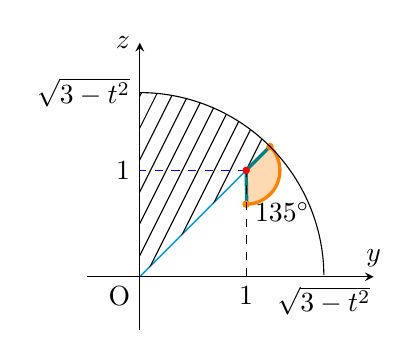
\begin{tikzpicture}[scale=1.35]
                            \fill [opacity=.3,orange] (1,1) -- ({sqrt(6)/2},{sqrt(6)/2}) -- plot [samples=500,domain={sqrt(6)/2}:{1-(sqrt(3)-sqrt(2))}] ({sqrt((sqrt(3)-sqrt(2))*(sqrt(3)-sqrt(2))-(\x-1)*(\x-1))+1},\x) -- cycle;
                            %\fill [opacity=.2] (0,0) -- ({sqrt(6)/2},{sqrt(6)/2}) -- plot [samples=500,domain={sqrt(6)/2}:0] (\x,{sqrt(3-\x*\x)});
                            \draw (0,0) -- (1.2,1.2);
                            \draw [cyan] (0,0) -- (1,1);
                            \begin{scope}
                                \path[clip] (0,0) -- ({sqrt(6)/2},{sqrt(6)/2}) -- plot [samples=500,domain={sqrt(6)/2}:0] (\x,{sqrt(3-\x*\x)});
                                \foreach \t in {1,2,...,50}{
                                  \path[draw,thin] (0.15*\t-1,0) -- (0.15*\t,2);
                                }
                              \end{scope}
                            \draw [very thick,teal] (1.006,{1-(sqrt(3)-sqrt(2))}) -- (1,1) -- ({sqrt(6)/2},{sqrt(6)/2});
                            \draw [very thick,orange,samples=500,domain={sqrt(6)/2}:{1-(sqrt(3)-sqrt(2))}] plot ({sqrt((sqrt(3)-sqrt(2))*(sqrt(3)-sqrt(2))-(\x-1)*(\x-1))+1},\x);
                            \fill [orange] ({sqrt(6)/2},{sqrt(6)/2}) circle(1pt);
                            \fill [orange] (1,{1-(sqrt(3)-sqrt(2))}) circle(1pt);
                            %\draw (1.2,1.2) coordinate (A) -- (1,1) coordinate (B) -- (1,0) coordinate (C) pic[draw=black, angle eccentricity=2.3, angle radius=0.3cm] {angle=C--B--A};
                            \draw (1.34,0.61) node {$135^\circ$};
                            \draw [samples=500,domain={1.732}:0] plot (\x,{sqrt(3-\x*\x)});
                            \draw [-stealth] (0,-0.5) -- (0,2.2) node [left] {$z$};
                            \draw [-stealth] (-0.5,0) -- (2.2,0) node [above] {$y$};
                            \draw ({sqrt(3)},0) node [below] {$\sqrt{3-t^2}$};
                            \draw (0,{sqrt(3)}) node [left] {$\sqrt{3-t^2}$};
                            \draw (1,0) node [below] {$1$};
                            \draw (0,1) node [left] {$1$};
                            \draw [dashed,blue] (1,1) -- (0,1);
                            \draw [dashed] (1,0) -- (1,1);
                            \draw (0,0) node [below left] {O};
                            \fill [red] (1,1) circle(1pt);
                        \end{tikzpicture}\\[2mm]
                        全体図 & $y=z$平面 & \begin{tabular}{c}$x=t$で切断した$yz$平面\\(斜線部は$V$の断面)\end{tabular}
                    \end{tabular}
                \end{table}

                %\begin{textblock*}{.4\textwidth}(190mm,160mm)
                %    \begin{tabular}{c}
                %        $t=\sqrt{3}\sin\theta\quad\therefore\,\,\bunsuu{dt}{d\theta}=\sqrt{3}\cos{\theta}$ \\[3mm]
                %        \begin{tabular}{|c|c|} \hline
                %            $t$ & $0\to1$\bsityuu \\ \hline
                %            $\theta$ & $0\to\alpha$\bsityuu \\ \hline
                %        \end{tabular}
                %    \end{tabular} \\[22mm]
                %    $\cos{\alpha}=\sqrt{1-\sin^2{\alpha}}=\bunsuu{\sqrt{2}}{\sqrt{3}}$ \\
                %    $\left(\because\,\,0<\alpha<\bunsuu{\pi}{2}\right)$
                %\end{textblock*}

                \noindent
                $U$の体積を求める。$U$の体積は$U_{\text{AB}}$の体積の4倍である。\textcolor{orange}{オレンジの網目部}は$y=z$平面上にあり,\textcolor{orange}{オレンジの網目部}と平面$x=t$の交線である図の\textcolor{teal}{緑線}について,その長さは,$\sqrt{3-t^2}-\sqrt{2}$となる。この\textcolor{teal}{緑線}を\textcolor{red}{線分AB}を回転の軸として$135^\circ$回転させた図形の面積は,
                \begin{align*}
                    \pi\cdot\left(\sqrt{3-t^2}-\sqrt{2}\right)^2\cdot\bunsuu{135}{360}=\bunsuu{3}{8}\pi\left(5-t^2-2\sqrt{2}\cdot\sqrt{3-t^2}\right)
                \end{align*}
                となる。これを$t$について$-1$から$1$まで積分すると,$U_{\text{AB}}$の体積が求まる。
                \begin{align*}
                    \bunsuu{3}{8}\pi\dint{-1}{1}\left(5-t^2-2\sqrt{2}\cdot\sqrt{3-t^2}\right)\,dt&=\bunsuu{3}{4}\pi\dint{0}{1}\left(5-t^2-2\sqrt{2}\cdot\sqrt{3-t^2}\right)\,dt \\
                    &=\bunsuu{3}{4}\pi\teisekibun{5t-\bunsuu{1}{3}t^3}{0}{1}-\bunsuu{3\sqrt{2}}{2}\pi\dint{0}{1}\sqrt{3-t^2}\,dt \\
                    &=\bunsuu{3}{4}\pi\left(5-\bunsuu{1}{3}\right)-\bunsuu{3\sqrt{2}}{2}\pi\dint{0}{\alpha}\sqrt{3-3\sin^2{\theta}}\cdot\sqrt{3}\cos{\theta}\,d\theta \\
                    &=\bunsuu{7}{2}\pi-\bunsuu{9\sqrt{2}}{2}\pi\dint{0}{\alpha}\cos^2{\theta}\,d\theta \\
                    &=\bunsuu{7}{2}\pi-\bunsuu{9\sqrt{2}}{2}\pi\dint{0}{\alpha}\bunsuu{1+\cos{2\theta}}{2}\,d\theta \\
                    &=\bunsuu{7}{2}\pi-\bunsuu{9\sqrt{2}}{2}\pi\teisekibun{\bunsuu{1}{2}\theta+\bunsuu{1}{4}\sin{2\theta}}{0}{\alpha} \\
                    &=\bunsuu{7}{2}\pi-\bunsuu{9\sqrt{2}}{2}\pi\left(\bunsuu{1}{2}\alpha+\bunsuu{1}{4}\sin{2\alpha}\right) \\
                    &=\bunsuu{7}{2}-\bunsuu{9\sqrt{2}\alpha}{4}\pi-\bunsuu{9\sqrt{2}}{4}\pi\sin{\alpha}\cos{\alpha} \\
                    &=\bunsuu{7}{2}\pi-\bunsuu{9\sqrt{2}\alpha}{4}\pi-\bunsuu{9\sqrt{2}}{4}\pi\cdot\bunsuu{1}{\sqrt{3}}\cdot\bunsuu{\sqrt{2}}{\sqrt{3}} \\
                    &=2\pi-\bunsuu{9\sqrt{2}\alpha}{4}\pi
                \end{align*}
                したがって,$U$の体積は,
                \begin{align*}
                    4\cdot\left(2\pi-\bunsuu{9\sqrt{2}\alpha}{4}\pi\right)=(8-9\sqrt{2}\alpha)\pi
                \end{align*}
                よって,求めるべき$W$の体積は,
                \begin{align*}
                    \bunsuu{2\sqrt{3}}{3}\pi+\bunsuu{20}{3}+(8-9\sqrt{2}\alpha)\pi=\boldsymbol{\left(\bunsuu{2\sqrt{3}}{3}+8-9\sqrt{2}\alpha\right)\pi+\bunsuu{20}{3}}\kotae
                \end{align*}
    \end{itemize}
\end{document}